\documentclass[]{IEEEtran}
\usepackage[utf8]{inputenc}
\usepackage[spanish,es-tabla]{babel}
\usepackage{amsmath}
\usepackage{amsfonts}
\usepackage{amssymb}
\usepackage{graphicx}
\usepackage{cite}
\usepackage{hyperref}
\usepackage{float}

\title{Procesamiento de imágenes utilizando Deep Learning y CARLA 
Simulator \\ 
Image processing with Deep Learning and CARLA Simulator}
\author{ 
Gatica, Isaias \\ { \small{isaiasgatica1@gmail.com} }\\ \and 
Saez, Lautaro Andres { \\ \small{lautaroandressaez@gmail.com } } }
\date{}

\providecommand{\keywords}[1]
{
  \small	
  \textbf{\textit{Keywords---}} #1
}

\begin{document}
    \maketitle

    \begin{abstract}
        En este informe se presenta la implementación de una red Pix2Pix capaz de pasar de una imagen RGB a 
        una imagen segmentada donde cada color indica un objeto diferente. Se comenzara desde cero obteniendo el 
        dataset medíante el simulador \textbf{CARLA} para luego poder entrenar la red con una gran variedad de imágenes con 
        diferente clima y vegetación. Finalmente se probara con imágenes reales para analizar la viavilidad de entrenar una 
        red con un simulador y luego ingresarla en el mundo real.
    \end{abstract}


    \begin{abstract}
        This report presents the implementation of a Pix2Pix network capable of going from an RGB image to
        a segmented image where each color indicates a different object. It will start from scratch obtaining the
        dataset using the \textbf{CARLA} simulator to then be able to train the network with a great variety of images with
        different climate and vegetation. Finally, it will be tested with real images to analyze the viability of training a
        network with a simulator and then enter it into the real world.
    \end{abstract}

    \keywords{Pix2Pix, CNN, GAN, RNN, NN, YOLO, SOM, \textbf{CARLA}}


    \section{Introducción}

    Con la intención de brindarle inteligencia a un automóvil, es necesario saber como éste se comunica con el mundo y cómo lo interpreta.
    Con el avance de la tecnología las cámaras toman preponderencia como sensores y combinando esta gran fuente de información (la fotografía) con un 
    algoritmo de segmentación las posibilidades de detección y decisión del vehículo parten de una buena base. 

    Pero, ¿cómo generar esta segmentación de forma automática y confiable? En los últimos años, debido a la necesidad de resolver problemás más complejos y la posibilidad de utilizar GPU's las redes neuronales han cobrado 
    gran importancia en nuetras vidas, y ya son parte del día a día, cosas tan simples como los filtros de Instagram basan 
    su reconocimiento facial en redes neuronales. 

    Las redes permiten resolver problemás que van desde la clasificación de imágenes hasta la conducción autónoma, claro está 
    que para esto existen diferentes arquitecturas las cuales son expecíficas para determinadas tareas, como el procesamiento de imágenes (CNN, GAN, YOLO), 
    procesamiento de texto (RNN), procesamiento de datos (NN).

    La desventaja principal de estos modelos supervisados es la necesidad de un dataset muy bien estructurado y para el cual es necesario 
    el trabajo humano, esta es la tarea más importante y que si está mal realizada la red no tendrá un desempeño correcto.

    Aquí es donde nace el uso de simuladores. En el paper \textit{Driving to Safety} \cite{Driving-to-safety}, se 
    plantean la siguiente situación ``los vehículos autónomos deberán ser conducidos cientos de millones de millas y, a veces, cientos de miles de millones de millas
    para hacer afirmaciones estadísticamente confiables sobre la seguridad''. Esto conlleva obviamente muchos gastos y riesgos, lo que un simulador reduce de gran 
    manera, no solo para la creación del dataset si no también para el posterior testeo de la conducción autónoma. 



    \section{Materias y metodos}

    En esta sección se detallan los recientes avances en los campos de interés.


    \subsection{\textbf{CARLA}}

    \textbf{CARLA} \cite{CARLA-Simulator} es un simulador de conducción el cual posee una API para Python lo que 
    permite de forma sencilla obtener datos del entorno. Esto permite una gran simpleza 
    a la hora de crear dataset o probar modelos de AI.
    
    \textbf{CARLA} cuenta con una gran variedad de sensores como GPS, LiDAR, cámaras RGB, cámaras de segmentación semántica, etc.
    También posee un ambiente muy variado, permiendo variaciones en la neblina, la hora del día e incluso el clima.

    \subsection{Deep Learning}

    Las redes neuronales son muy utilizadas en el campo de la minería de datos, debido a 
    su gran versatilidad. Dentro de este mundo existen 2 grandes tipos de entrenamientos: 
    los supervisados, que dada una entrada $X$ se conoce la salida deseada $Y$, y 
    los algoritmos no supervisados, como los modelos de Q-learning o los mapas autoorganizados (SOM).
    En este proyecto se optó por un entrenamiento supervisado.

    
    Para el modelado de la red neuronal se utilizó un modelo llamado Pix2Pix \cite{Pix2Pix},
    el cual pertime dada una imagen de entrada $X$ obtener una imagen de salida $Y$.

    Este modelo consta de $2$ redes separadas, la primera es denominada generador Fig.\ref{fig:generator}
    el cual deberá aprender a segmentar la imagen semánticamente. Y la segunda se llama discriminador Fig.\ref{fig:discr}
    este se encarga de corregir al generador aprendiendo cuando una salida es ``realista". 
    Llamaremos salida \textit{realista}  a aquella imagen que cumpla el objetivo esperado, en este caso sería una imagen segmentada 
    de forma coherente.
    
    \begin{figure}
        \centering
        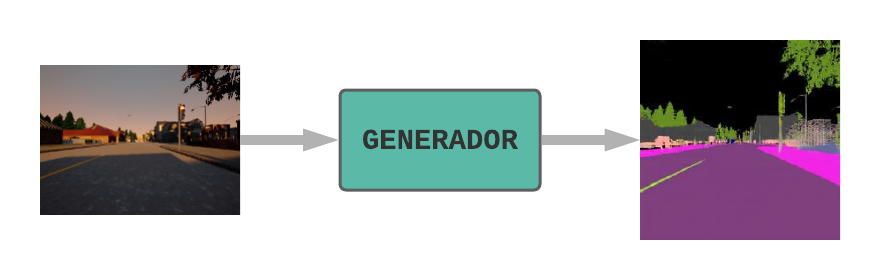
\includegraphics[width=.4\textwidth]{Imgs/Generador.png}
        \caption{Esquema de la red generativa.}
        \label{fig:generator}
    \end{figure}

    \begin{figure}
        \centering
        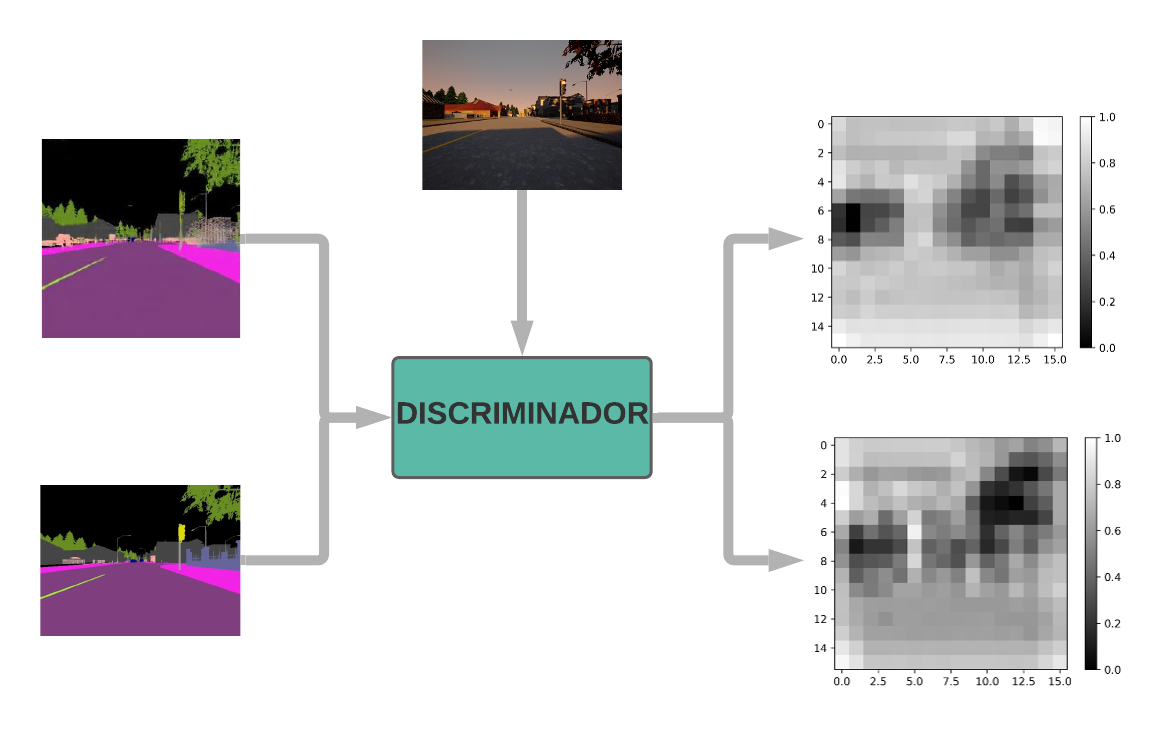
\includegraphics[width=.4\textwidth]{Imgs/Discriminador.png}
        \caption{Esquema de la red discriminativa.}
        \label{fig:discr}
    \end{figure}
    


    \subsubsection{Generador}
    
    El generador cuenta con una arquitetura denomina U-net \cite{U-Net},  
    la cual posee una muy buena eficiencia debido a los bypass que existen entre las capas de convolución y 
    las capas de deconvolución. Con la finalidad de comprender de forma más sencilla se puede observar 
    en la Fig.\ref{fig:u-net} dicha arquitectura.

    \begin{figure}
        \centering
        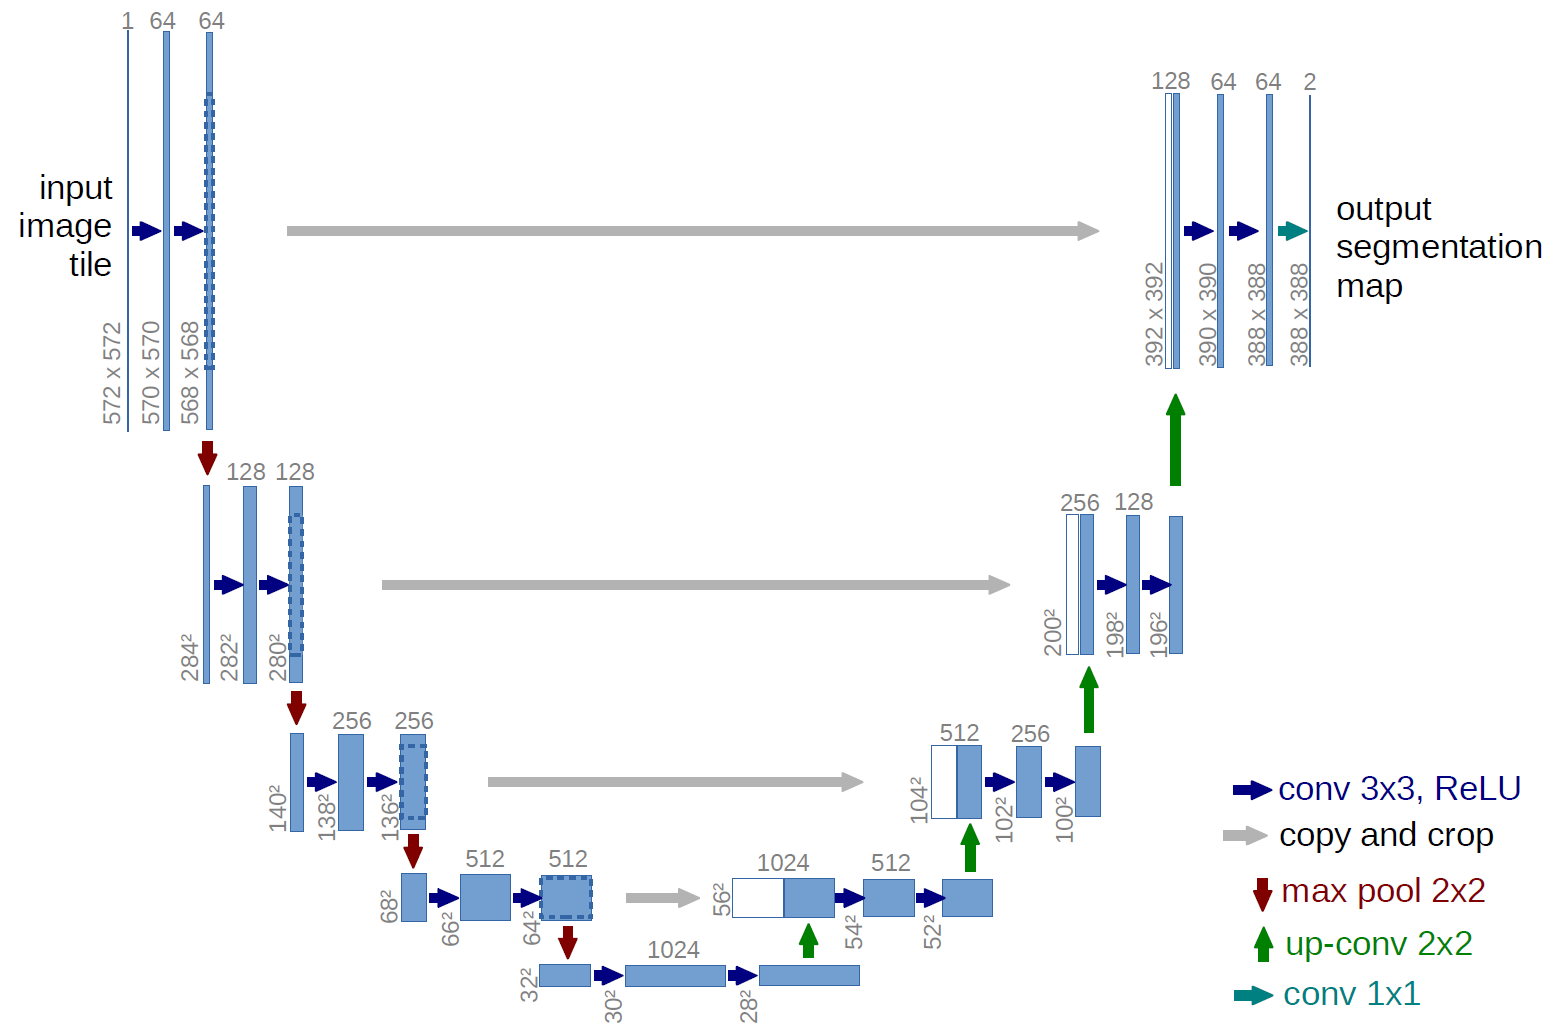
\includegraphics[width=.4\textwidth]{Imgs/u-net-architecture.png}
        \caption{Arquitectura de una U-net.}
        \label{fig:u-net}
    \end{figure}

    El error del generador es cuantizado por la red discriminativa.

    \subsubsection{Discriminador}

    El discriminador posee una arquitectura mucho más sencilla, la cual consta de $6$ capas de convolución.
    Esto se debe a que la salida representa qué tan realista es un segmento de la imagen de entrada. 
    El error del discriminador se cuantifica medíante una entropía cruzada. Ya que 
    se propone que siempre que le entre una imagen del generador la salida debe ser una matriz de $0$, ya que 
    esta imagen no es del dataset, mientras que cuando la entrada sea una imagen del dataset el resultado debe ser un $1$. 
    
    Esto desemboca en una pelea entre en generador, ya que debe aprender a engañar al discriminador 
    , y el discriminador, que debe lograr siempre reconocer que la imagen $\hat{Y}$ es totalmente falsa, ya que es una 
    creación de la red generativa.
 
    \subsection{Preprocesado de datos}

    Un paso fundamental para trabajar con algoritmos de imágenes es pasar del domininio $[0;255]$ a 
    un dominio más acotado, para este trabajo se utilizó el dominio de $[-1;1]$. De esta forma se logra 
    una mayor eficiencia computacional.

    Debido al tamaño de las imágenes es recomendable hacer un resize a dimensiones más pequeñas 
    para disminuir el uso de RAM cuando son cargadas en memoria y el uso de GPU al realizar las convoluciones. En 
    este caso las imágenes de entrada y de salida son redimensionadas a $256x256$.

    \subsubsection{Random jitter}

    El \textit{random jitter} es un proceso por el cual se busca realizar un aumentado
    del dataset, esto disminuye la posibilidad de experimentar \textbf{overfitting}. 
    Este proceso cuenta de $2$ pasos:

    \begin{itemize}
        \item[Crop] Se realiza un resize a $286x286$ para luego realizar un recorte a $25x256$.
        \item[Flip] De forma aleatoria con probabilidad $0.5$ se realiza un rotación de $180^\circ$. 
    \end{itemize}

    Debido a que es utilizan en algoritmos supervisados es necesario aplicar 
    el \textit{random jitter} tanto a la imagen de entrada como a la de salida,
    para ello se hace un stack de las mismás como se observa en la Fig.\ref{fig:random-jitter}.

    \begin{figure}
        \centering
        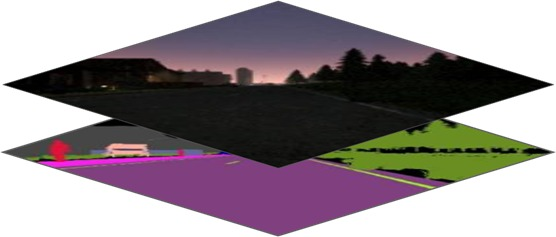
\includegraphics[width=.4\textwidth]{Imgs/stack-random-jitter.jpeg}
        \caption{Visualización del stack previo al random jitter.}
        \label{fig:random-jitter}
    \end{figure}

    En la Fig.\ref{fig:crop-flip} se observa el proceso de random jitter completo.

    \begin{figure}
        \centering
        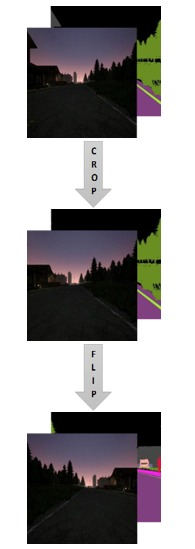
\includegraphics[width=.25\textwidth]{Imgs/random_jitter.jpeg}
        \caption{Visualización del random jitter.}
        \label{fig:crop-flip}
    \end{figure}

    \section{Propuesta}

    Se propone realizar una red neuronal utilizando la arquitectura Pix2Pix que 
    aprenda a segmentar semánticamente una imagen. Adicionalmente el 
    dataset utilizado será obtenido medíante \textbf{CARLA} permitiendo de esta forma 
    pasar por todo el trayecto del diseño de una red que resuelve un nuevo problema. 
    Este proceso consta de 

    \begin{enumerate}
        \item Definir la arquitectura a utilizar.
        \item Crear un dataset útil para solucionar el problema.
        \item Entrenar la red.
        \item Testear el rendimiento de la misma.
        \item Realizar mejoras a la arquitectura para obtener alguna de las siguientes ventajas: 
            \subitem Mayor velocidad de procesado.
            \subitem Mejor rendimiento. 
            \subitem Eliminar el overfitting o underfitting si existiera.
        \item Repetir los pasos anteriores hasta lograr un resultado satisfactorio.
    \end{enumerate}

    \section{Pruebas y resultados}

    Se presentará de forma ordenada todas las etapas del proyecto. 
    Debido a la cantidad de imágenes utilizadas no es posible presentarlas a todas, por ello 
    se relizarán análisis particulares para algunos casos de interés.

    \subsection{Obtención del dataset}

    Para obtener el dataset se colocaron una camara RGB y una camara de segmentación semántica
    \cite{CARLA-Sensors-Reference}, ubicadas en la misma posición. Se recolectaron los datos 
    cada 5 segundos. Las condiciones climáticas utilizadas fueron aleatorias, por lo que se logra
    obtener un dataset mucho más variado, una representación de esté puede observase en 
    Fig.\ref{fig:dataset}.

    \begin{figure}
        \centering
        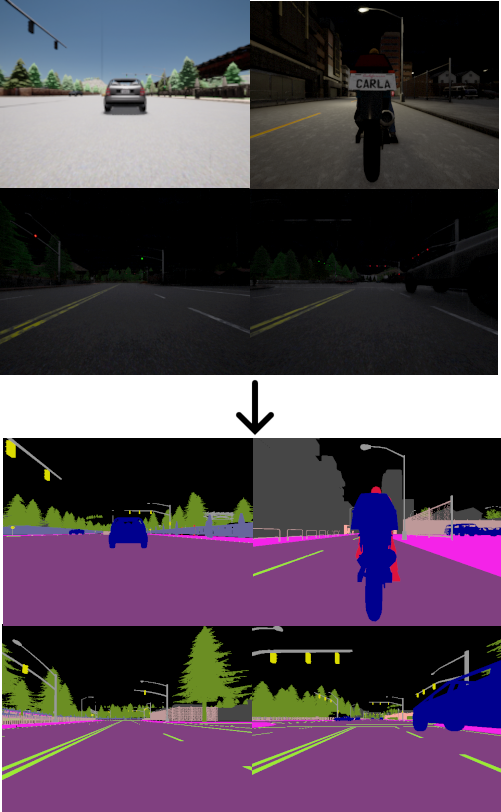
\includegraphics[width=.5\textwidth]{Imgs/Dataset.png}
        \caption{Imágenes de muestra del dataset}
        \label{fig:dataset}
    \end{figure}

    Para lograr un manejo autónomo del vehículo se utilizó el autopilot \cite{CARLA-Documentation}. 
    Con la finalidad de aumentar la variedad de imágenes se utilizaron todos los mapas posibles y 
    se adicionaron otros vehículos autónomos junto a personas. aúnque debido 
    a limitaciones de hardware solo se pudieron ingresar 20 personas, lo cual 
    provocó una deficiencia en la detección de personas de la red Pix2Pix. 

    \subsection{Entrenamiento de la red}

    Como fue mencinado en el marco teórico el modelo implementado se denomina Pix2Pix \cite{Pix2Pix}.
    Se utilizó como entrada la imagen de la camara RGB y la salida será una imagen segmentada, para ello se utilizó
    el dataset obtenido con el simulador de \textbf{CARLA} el cual posee 8000 imágenes. 

    \subsubsection{Tratamiento de las imágenes}

    Para evitar problemás en el entrenamiento de la red es muy usual llevar los valores de cada canal al 
    intervalo $[-1;1]$, esto evita problemás de continuidad en la red. Luego 
    se procede a aplicar un \textit{random jitter}.

    El dataset fue dividido en 2 partes, una utilizada para el entrenamiento, aproximadamente el $80 \% $ de las imágenes, y la 
    otra parte para el testing de la red utilizando el $20 \%$ restante, siguiendo el principio de Pareto.

    \subsubsection{Entrenamiento}

    Para realizar el entremiento se utlizó el dataset de testing, aproximadamente 6400 imágenes, 
    y se realizaron 400 iteraciones a la red para lograr un mejor desempeño. A continuación se muestran 2 
    casos de interés debido a la gran densidad del dataset de testing.
    
    En la Fig.\ref{fig:results}
    se muestra una comparación para $1$ imagen del dataset de testing luego de la primera iteración 
    y al finalizar el entrenamiento.
    Puede observarse que existieron grandes mejoras sobre todo en la zona de la palmera
    donde, al finalizar el entrenamiento, es posible observar los detalles de la misma.
    aúnque cabe destacar que debido a la poca cantidad de señales de tráfico en el dataset
    se observa que si bien reconoce la estructura del semáforo no es capaz de utilizar el color 
    adecuado.

    \begin{figure}[htb]
        \centering
        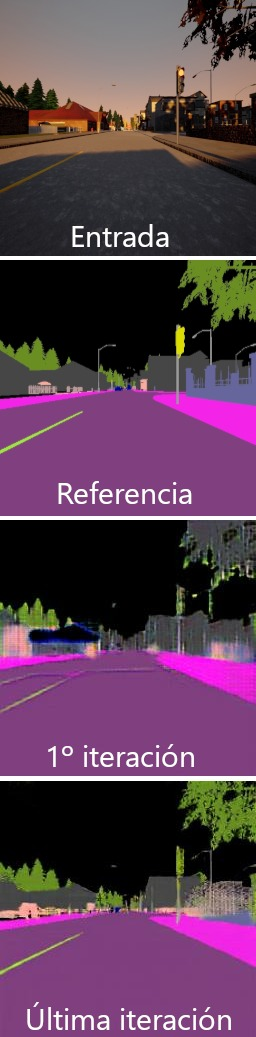
\includegraphics[width=.25\textwidth]{Imgs/results.jpeg}    
        \caption{Imagen del dataset de testing con señal de tráfico.}
        \label{fig:results}
    \end{figure}

    Al analizar otro imagen del dataset la cual se observa en la Fig.\ref{fig:person_image}
    se puede ver que la persona no es detectada, esto se le atribuye a la poca densidad de imágenes con personas 
    que había en el dataset.

    \begin{figure}
        \centering
        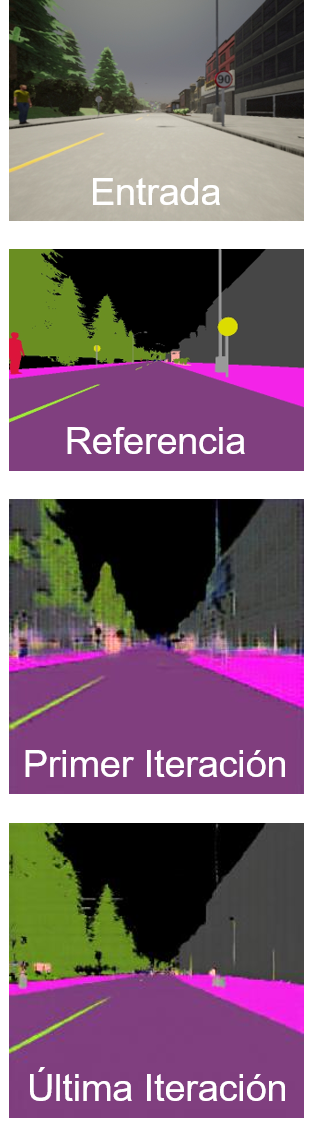
\includegraphics[width=.25\textwidth]{Imgs/results-2.png}
        \caption{Imagen del dataset de testing con persona.}
        \label{fig:person_image}
    \end{figure}

    \subsection{Imágenes reales}

    En este apartado se muestran 2 imágenes de interés para mostrar el comportamiento del modelo entrenado en situaciones reales.

    En la Fig.\ref{fig:real-results} se observa como para un cielo despejado la red es capaz de detectar de forma muy eficiente los límites. 
    Al analizar la palmera se observa un resultado muy similar. Pero para zonas con mayor detalle se observa una deficiencia de la red, tal 
    como sucede con los autos o los arbustos del lado izquierdo. Por otro lado en la Fig.\ref{fig:real-results2} como el cielo esta nublado 
    la red tiene grandes problemás para delimitar las fronteras. aúnque se observa un buen resultado en la delimitación de los árboles del fondo, 
    si bien el color no es el adecuado la red logra detectar las señales de tráfico en ambas imágenes.

    \begin{figure}[htb]
        \centering
        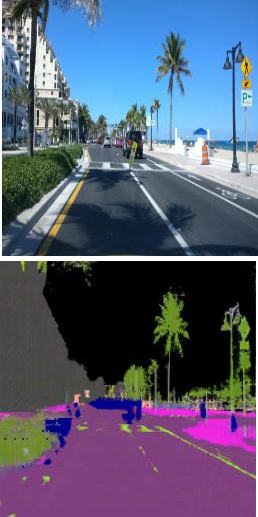
\includegraphics[width=.4\textwidth]{Imgs/PalmeraRGBSEM.png}    
        \caption{Imagen real y su respectiva segmentación semántica por la red luego del entrenamiento.}
        \label{fig:real-results}
    \end{figure}
    \begin{figure}[htb]
        \centering
        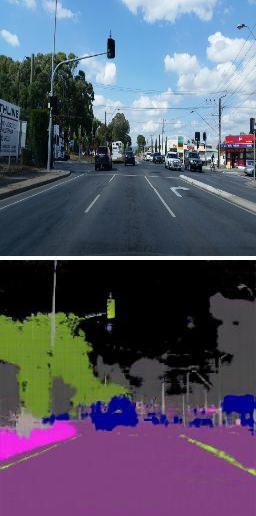
\includegraphics[width=.4\textwidth]{Imgs/SemaforoRGBSEM.png}    
        \caption{Imagen real junto a su representación segmentada por la red.}
        \label{fig:real-results2}
    \end{figure}

    \section{Conclusiones}
    
    Al analizar los resultados del modelo con las imágenes que se obtienen desde el simulador se observa un desempeño correcto. aún que 
    existen ciertos detalles tales como: personas, señales de tránsito y paradas de colectivo. Estos problemás se adjudican a la poca 
    densidad de estos en el dataset de training. En el caso de las personas existe una limitación por parte del simulador ya que no 
    deja ingresar más de $20$. Los otros problemás son asociados a los mapas y la cantidad de señales de tráfico que estos presentan, una 
    posible solución sería aumentar el tamaño del dataset o utilizar una red especializada en detección de señales de tráfico.

    Para las imágenes reales si bien el desempeño de la red disminuye y se observan otros problemás como las nubes los resultados generales 
    dan esperanza sobre futuras redes entrenadas en simuladores para luego pasarlas a un entorno real. Un gran problema y que aún no 
    ha sido solucionado es la iluminación, debido a su alta complejidad. Estas diferencias entre la realidad y el simulador desemboca 
    en regiones que no son delimitadas de forma correcta y colores erróneos. aúnque las regiones de mayor interés son detectadas como 
    la calle, la vereda y los autos, pero no bien delimitadas. Esto nos permitiria realizar una aproximación de donde se ubican los puntos 
    de interés como otros vehículos.


    \subsection{Ventajas}

    A continuación se nombrarán algunas ventajas de realizar la segmentación semántica, en particular con un simulador y una red Pix2Pix. 
    Ordenadas según importancia decreciente:
    
    \begin{enumerate}
        \item Posibilidad de reconocer objetos o zonas de una forma
        mucho más sencilla. 
        \item Al utilizar un simulador, la principal ventaja recae en la posibilidad de crear un dataset con el mínimo esfuerzo humano, tiempo y costo monetario.
        \item Gran flexibilidad de simular situaciones externas o propias del
        vehículo mientras se recolectan datos. Permitiendo simular situaciones anómalas.
        \item Al utilizar redes neuronales no existe una etapa de diseño de descriptores, ya que estos son obtenidos por la red.
        \item Reducción del tiempo de procesado de información.
        \item Las imágenes semánticas ocupan menos espacio en memoria que su equivalente en RGB.
    \end{enumerate}
    
    \subsection{Desventajas}
    
    Por otro lado al analizar las desventajas de este modelo con el mismo criterio obtenemos:
    
    \begin{enumerate}
        \item Existe una diferencia significativa entre el entorno simulado y el real.
        \item Limitaciones de las computadoras actuales para realizar procesos de simulación y entrenamiento de forma simultánea.
        \item Alto costo computacional.
        \item Para problemás de alta complejidad y modelos de gran densidad es necesario datasets de gran tamaño.
        \item Tiempo de generado del dataset.
    \end{enumerate}


    Finalmente, estas practicas son de suma importancia en la actualidad debido a que permiten entrenar modelos por costos mucho menores. 
    Adicionalmente se debido a la revolución de las redes neuronales a partir del 2009 y el aumento en la demanda de modelos para resolver todo 
    tipo de tareas hoy en día es muy necesario la reducción de costes y de tiempos de creación tanto del dataset como el proceso de entrenamiento del modelo. 
    Si bien los resultados obtenidos para imágenes reales todavia no estan cerca de poder reemplazar los obtenidos con dataset de imágenes reales, se 
    observan resultados aceptables.

 
    \bibliographystyle{IEEEannot}
    \bibliography{biblio}
\end{document}